\section{8. Behaviour}

\subsection{8.1 Key scenario: ventilating ahead of a fika break}

\begin{figure}[H]
\centering
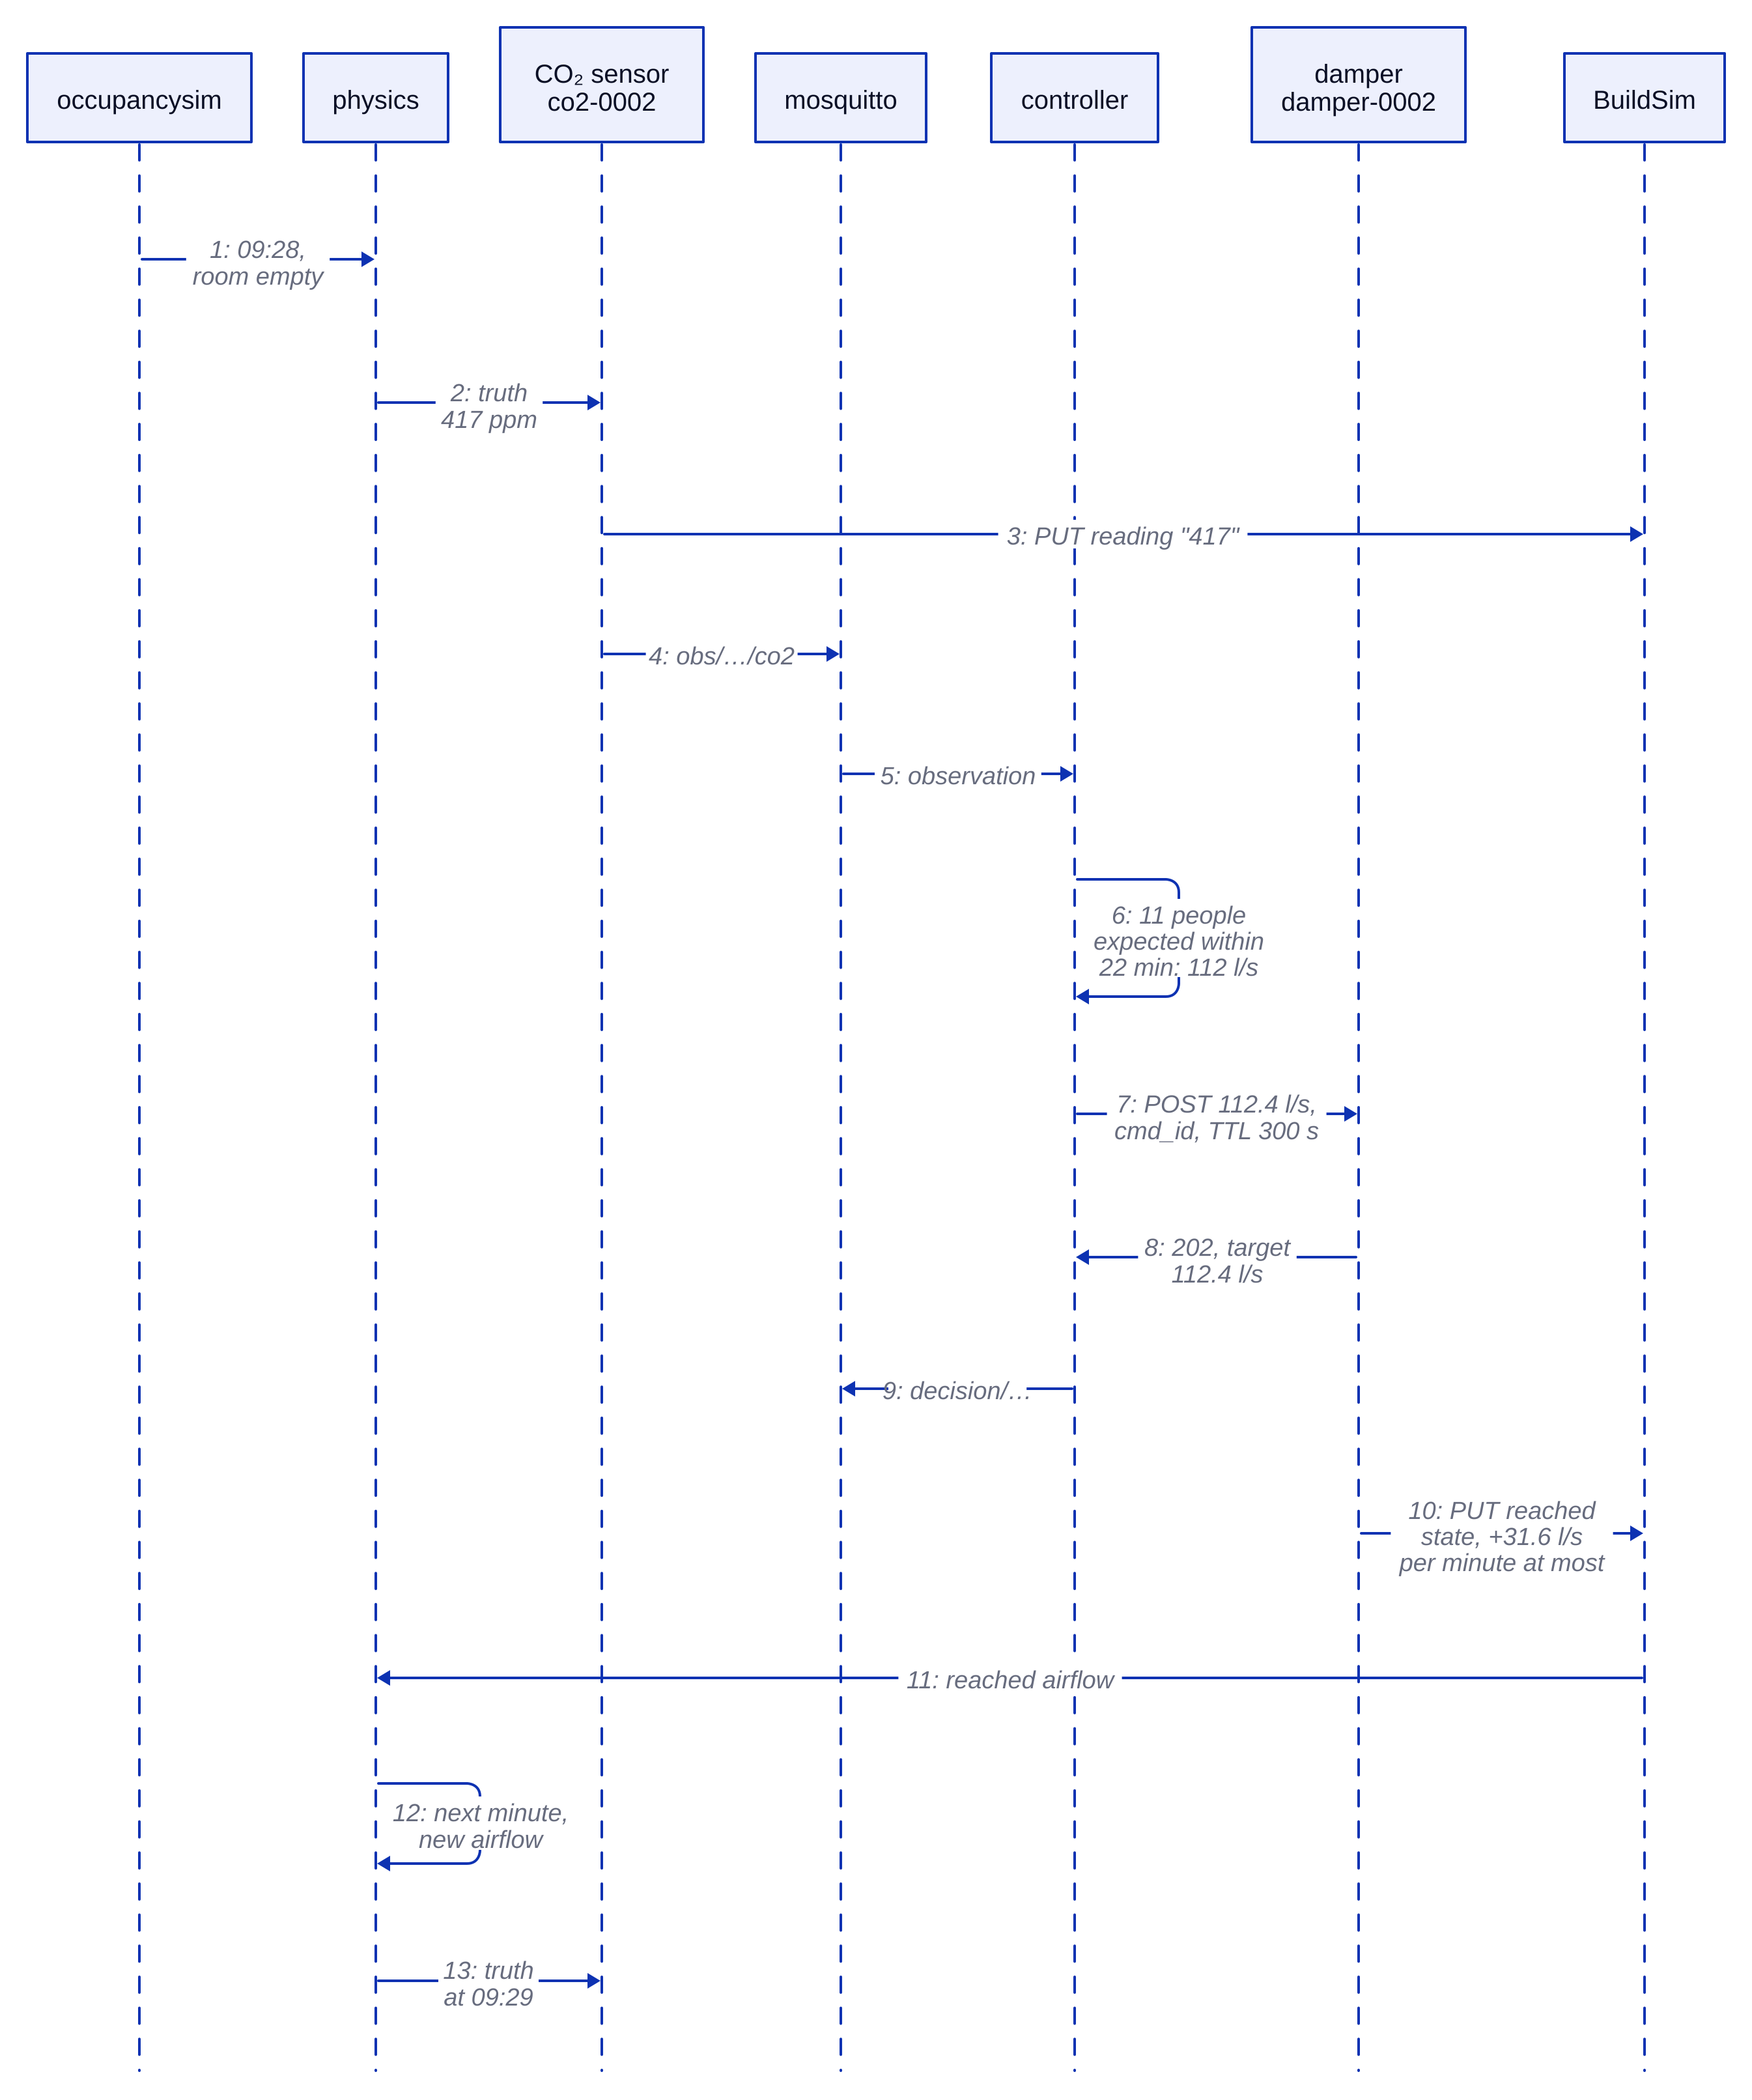
\includegraphics[width=\linewidth]{figures/dynamic.png}
\caption{One control period in fika room 1570 under the predictive policy, at
09:28, about twenty minutes before the morning break. The numbers are from a
run of 2026-09-30.}
\label{fig:dynamic}
\end{figure}

The room is empty and its air is clean, so the reactive term asks for the
minimum. What raises the airflow is step 6: the profile says that about 11
people are usually here within the room's lead time of 22 minutes, and the
workplace rule gives $7\times 11 + 0.35\times 101 = 112$~l/s for them. The
command (step 7) carries an id, the model time of the reading it was decided
on, and a time to live. The damper answers at once with the target it accepted
(step 8) and then travels towards it at no more than a tenth of its maximum
per model minute, writing each state it reaches to BuildSim (step 10). Physics
reads that state on its next tick (step 11), and from the next model minute
the room is computed with more air (step 12). When the people arrive at about
09:45 the damper is already open.

Three properties of this sequence matter for failures:
\begin{itemize}
\tightlist
\item Steps 3 and 4 are two writes. If the broker is down, step 3 still
  happens, and the controller and the damper find the reading in BuildSim.
\item Step 8 is synchronous. The controller knows whether its command was
  accepted, clamped or refused before it records the decision in step 9.
\item Nothing after step 7 needs the controller. If it dies there, the damper
  carries the command out and holds it for 300~s, then returns to design flow.
\end{itemize}

\subsection{8.2 Process lifecycle: a damper actuator}

\begin{figure}[H]
\centering
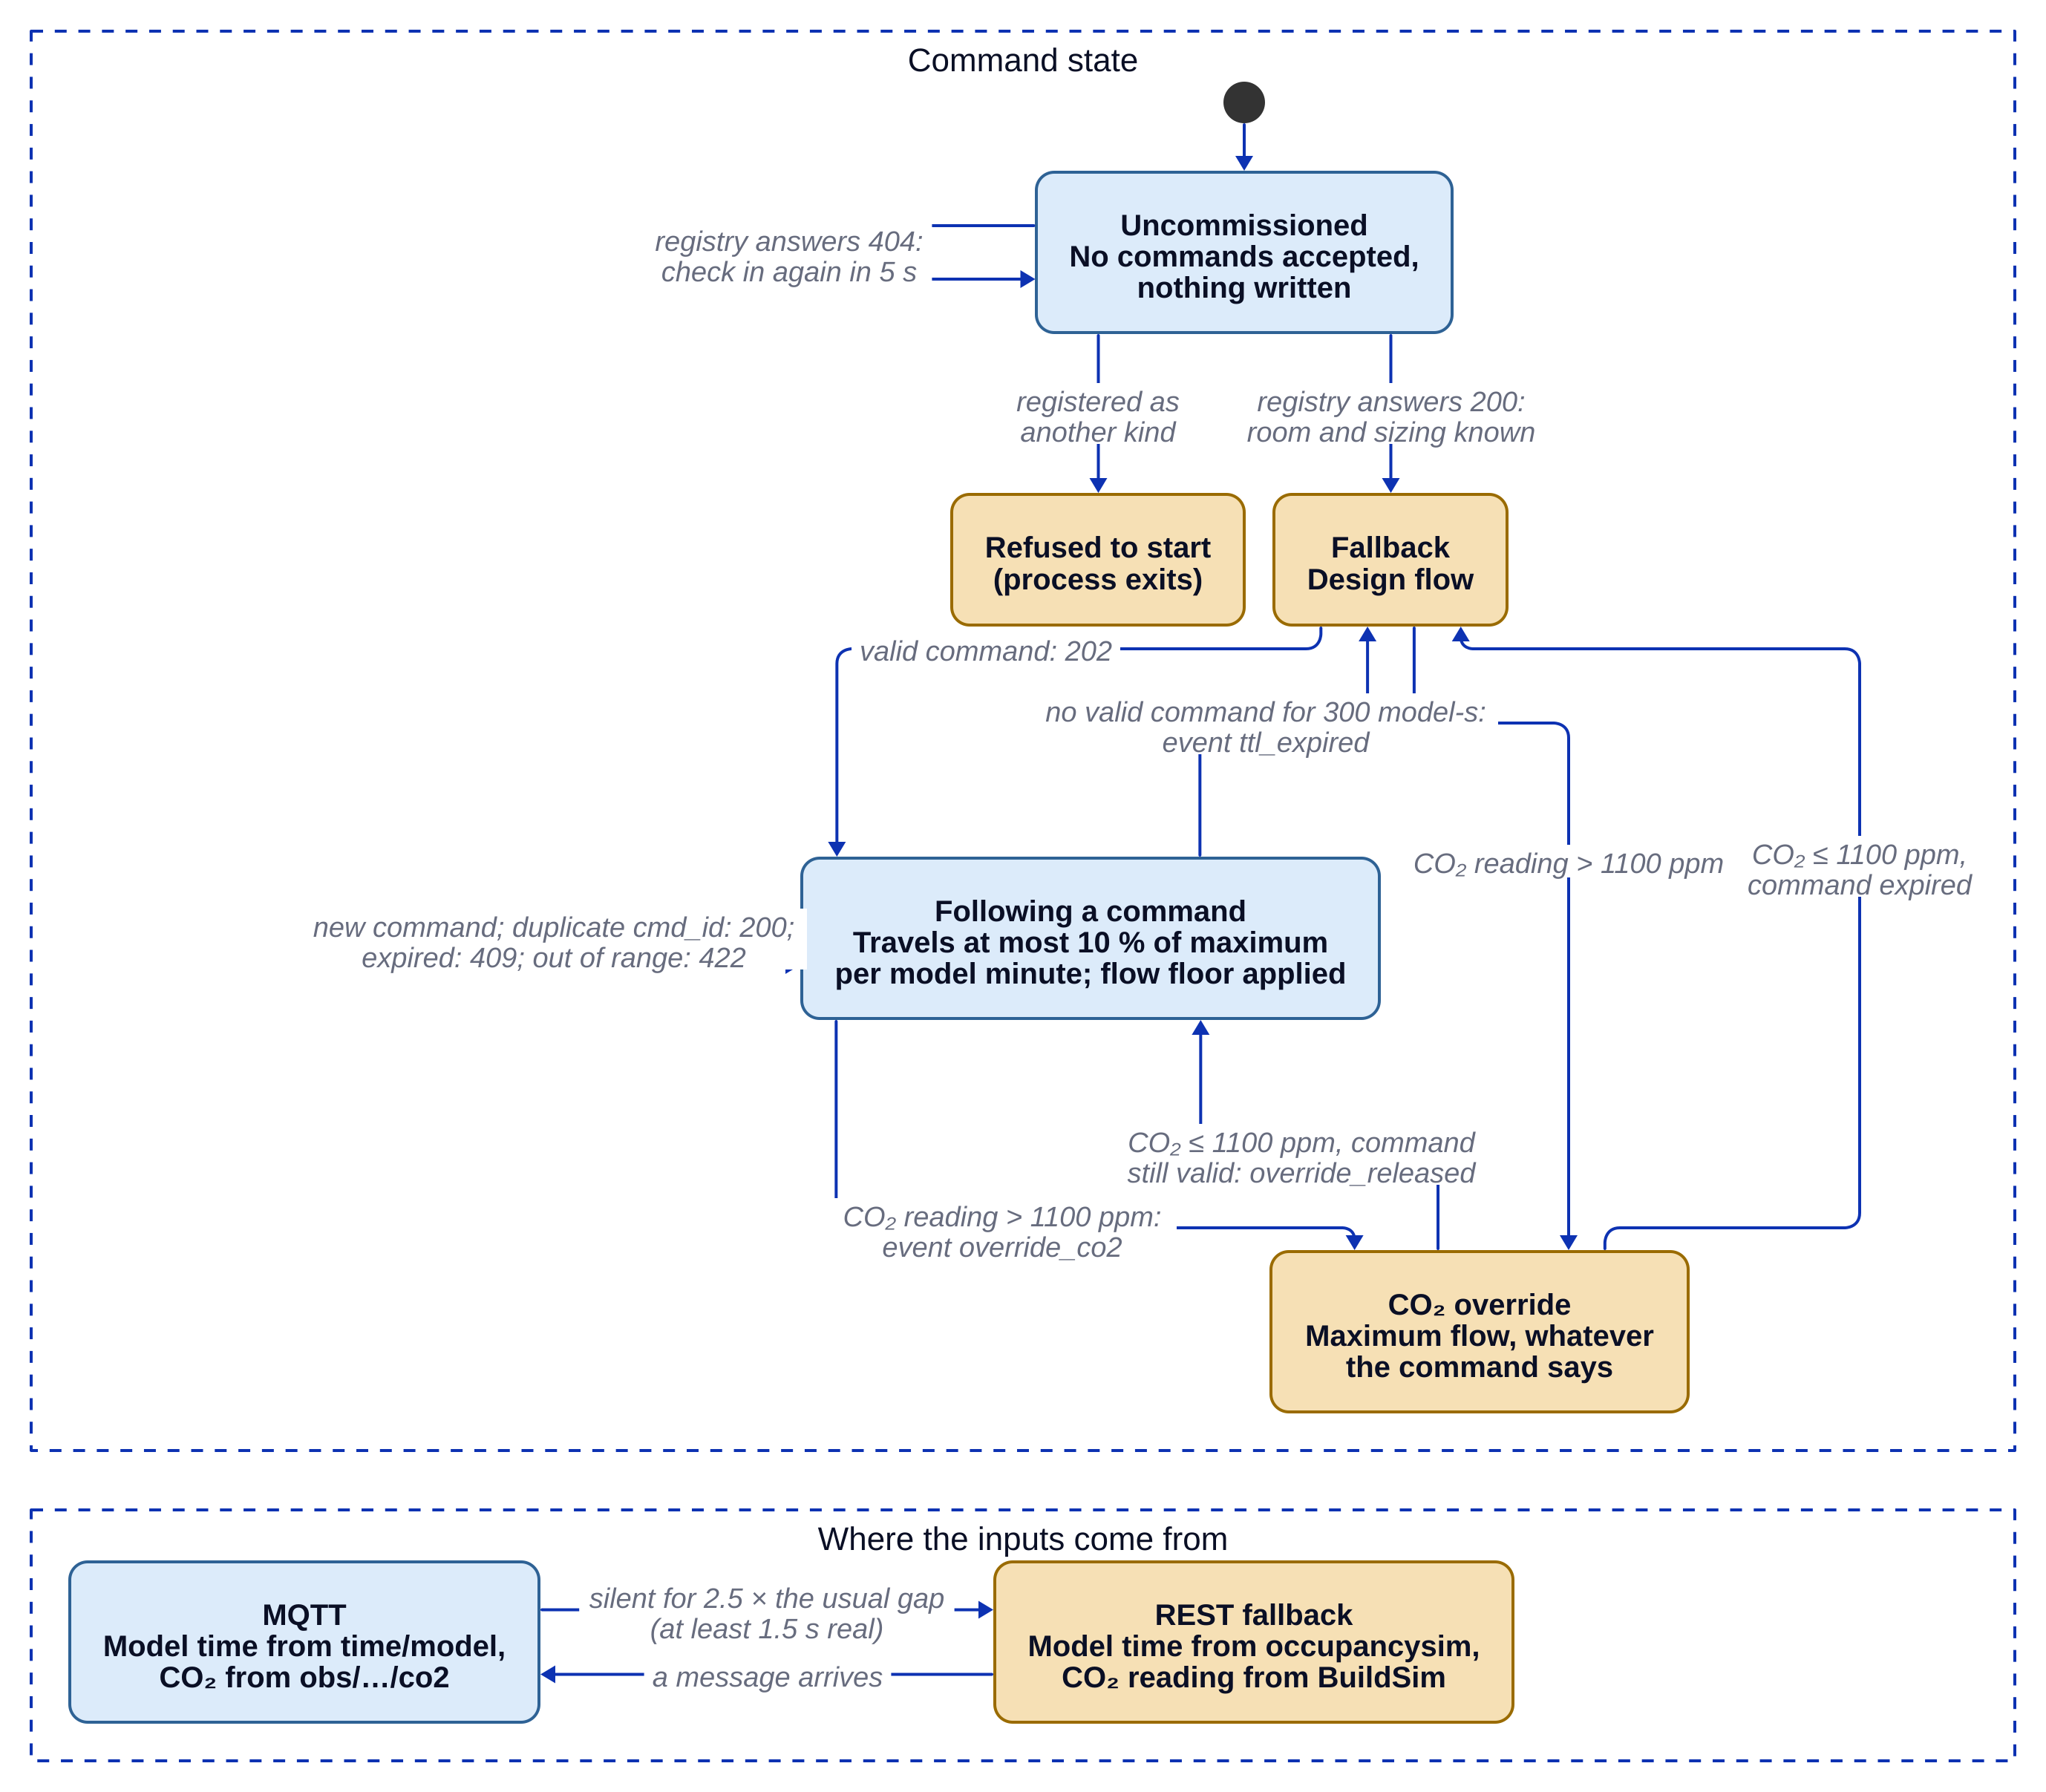
\includegraphics[width=0.86\linewidth]{figures/state.png}
\caption{States of one damper actuator. Blue states are normal operation,
yellow ones are fallbacks. A radiator valve is the same without the override,
and its fallback is 21~°C.}
\label{fig:state}
\end{figure}

\textbf{Start-up.} A device knows only its id and what kind of hardware it is.
It asks the registry every 5~s real until an installer has registered it, and
does nothing else in the meantime. If the registry says it is another kind of
device, it refuses to start, so a mistyped entry cannot make a damper act as a
valve. Once it knows its room and the room's sizing it starts in the fallback,
at design flow.

\textbf{Commands.} A valid command moves it to \emph{following}. Each further
command is checked again. If none arrives for the command's time to live, the
actuator publishes \code{ttl\_expired} and returns to the fallback. This one
transition covers a dead controller, a silent \COtwo{} sensor and a lost
network path between them, without the actuator having to tell them apart.

\textbf{Override.} From either state, a \COtwo{} reading above 1100~ppm opens
the damper fully and publishes \code{override\_co2}. Commands are still
received and remembered during an override, but the target stays at the
maximum until a reading is back at or below 1100~ppm.

\textbf{When the network drops.} The actuator takes the model time and the
room's \COtwo{} from the broker. If either goes silent, for 2.5 times the usual
gap between messages and at least 1.5~s real, it asks occupancysim for the
time and BuildSim for the reading instead, and returns to the broker as soon as
a message arrives. Without any source of time it keeps its current target and
cannot expire a command; that is the one situation in which a stale command
outlives its time to live. If BuildSim restarts, the actuator's writes are
refused until the registry has recreated its equipment, at most 10~s real, and
then continue.

The command, fallback and override transitions are branches in
\code{internal/actuator}, each with a unit test (T-07 to T-11). The start-up
transitions are covered by the commissioning tests (T-28 to T-31).
